\textbf{10.1.} 一漏电电容器的平板之间的空间填满电阻为 $5.0 \times 10^{5} \Omega$ 的物质, 电容器的电容是 $2.0 \times 10^{-6} \mathrm{~F}$ , 它的极板是圆形的, 半径为 $30 \mathrm{~cm}$ , 内部电场均匀, 在 $t = 0$ 时刻, 电容器两端的初始电压是零.

(1) 如果电压以恒定速率 $1.0 \times 10^{3} V \cdot s^{-1}$ 增加, 那么位移电流是多少?

(2) 通过电容器的真实漏电流在什么时间等于位移电流?

(3) 在半径 $r = 20\mathrm{cm}$ 处，在 $t = 0, 1.0, 2.0\mathrm{s}$ 时刻，极板之间的磁场大小各是多少？

\vfill

\textbf{10.2.} 设一导线的电导率为 $\sigma$ ，介电常量近似等于真空介电常量 $\varepsilon_{0}$ ，通以角频率 $\omega$ 的交流电.

(1) 导线中传导电流与位移电流之比是多少?

(2) 已知铜的电导率 $\sigma=5.9\times10^{7}\Omega^{-1}\cdot m^{-1}$ ，分别计算铜导线载有频率为 50Hz 和 $3.0\times10^{11}Hz$ 的交流电时，传导电流密度与位移电流密度的大小之比.

\vfill

\newpage

\textbf{10.3.} 一平行板电容器的两板均为半径为 $a$ 的圆板，接于一交流电源，板上电量的变化为 $Q = Q_{0}\sin \omega t$ ，试求两板之间 $(r < a)$ 和外部的磁场强度.

\vfill

\textbf{10.4.} 两种各向同性介质相接，它们的介电常量和磁导率分别为 $\varepsilon_{1}, \mu_{1}$ 和 $\varepsilon_{2}, \mu_{2}$ . 设交界面上无自由电荷和传导电流，在交界面两边，电场强度和交界面法线的夹角分别为 $\theta_{1}$ 和 $\theta_{2}$ ，磁场强度与交界面法线的夹角分别为 $\varphi_{1}$ 和 $\varphi_{2}$ ，见习题10.4图. 证明：
\begin{eqnarray*}
    \varepsilon_ {1} \cot \theta_ {1} &= \varepsilon_ {2} \cot \theta_ {2}  \\
\mu_ {1} \cot \varphi_ {1} &= \mu_ {2} \cot \varphi_ {2}
\end{eqnarray*}

\begin{center}
    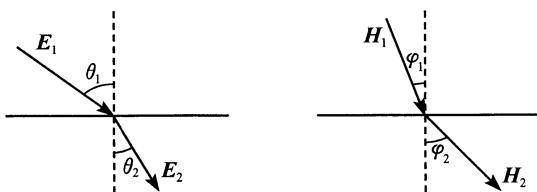
\includegraphics[width=0.5\linewidth]{figures/fig_10_4.jpg}
\end{center}

\vfill

\newpage

\textbf{10.5.} 频率为 $5 \times 10^{9} Hz$ 的电磁波在某介质中传播, 其电场强度的振幅为 $10 mV \cdot m^{-1}$ . 设介质的相对介电常量为 2.53, 相对磁导率为 1. 试求

(1) 传播速度;

(2) 波长；

(3) 磁场强度的振幅.

\vfill

\textbf{10.6.} 一个频率为 $7.94 \times 10^{7} \mathrm{~Hz}$ 的无线电波在距离发射机 $100 \mathrm{~km}$ 处的电场强度振幅为 $E = 15 \mathrm{mV} \cdot \mathrm{m}^{-1}$ . 我们假设发射机在各个方向上传送的功率均匀. 求

(1) 在该点的磁场强度振幅 H;

(2) 波数 k;

(3) 波长 $\lambda$ ;

(4) 发射机发射的功率 P.

\vfill

\newpage

\textbf{10.7.} 一条圆柱状导线, 其截面是半径为 $a$ 的圆, 其电阻率为 $\rho$ , 通过恒定的电流 $I$ . 求导线内部距离轴为 $r$ 处的 $E, H$ 和坡印廷矢量 $S$ 的大小和方向, 并将坡印廷矢量大小与长度为 $l$ , 半径为 $r$ 的导体体积内能量的耗散率进行比较.

\vfill

\textbf{10.8.} 在地球轨道上太阳辐射的平均强度(即平均能流密度)是 $\bar{S}=1353W\cdot m^{-2}$ ，太阳半径约为 $R_{0}=7\times10^{8}m$ ，太阳到地球的距离约为 $d=1.5\times10^{11}m$ .

(1) 求在太阳表面处太阳辐射的平均强度 $\overline{S}_{0}$ ;

(2) 求在太阳表面处电场强度的有效值；

(3) 求在太阳表面处磁场强度的有效值.

\vfill

\newpage

\textbf{10.9.} 强度为 S 的光入射到一镜子上, 入射光线与镜子平面法线成 $\theta$ 角.

(1) 光线对镜子压力 p 多大?

(2) 如果入射光能被镜子吸收的份额为 a，那么压力 p 是多少？

\vfill

\textbf{10.10.} 一球形电容器，内外半径为 $r_1, r_2$ ，带电为 $Q$ ，自转转动惯量为 $I$ ，静置于一均匀磁场 $\pmb{B}$ 中，当将 $\pmb{B}$ 撤销时，求电容器自转角速度的大小